\chapter{Juin 2021}

\paragraph{Question 1} \textit{Oscillateur harmonique quantique.} \\

Considérons un oscillateur harmonique de pulsation propre $\omega$. En unités sans dimensions ($\hbar=1$), les opérateurs position $\hat X$ et impulsion $\hat P$ obéissent à la relation de commutation canonique $[\hat X, \hat P]=i $. \\

Les opérateurs de création et destruction sont définis par 
$\hat a= \frac{1}{\sqrt{2}}(\hat X+i\hat P)$, $a^\dagger= \frac{1}{\sqrt{2}}(\hat X-i\hat P)$ et satisfont donc $[\hat a,\hat a^\dagger]=1$. \\

L'opérateur nombre $\hat N$ est donné par $\hat N= \hat a^\dagger \hat a$ et ses vecteurs propres sont notés $\hat N \ket{n} =n \ket{n}$ où $n \in \mathbb{N}$. On peut montrer que $\hat a \ket{n} =\sqrt{n} \ket{n-1}$ et que $\hat a^\dagger \ket{n} =\sqrt{n+1} \ket{n+1}$. L'hamiltonien de l'oscillateur harmonique est $\hat H = \frac{1}{2}\omega ( \hat P^2 + \hat X^2 )\ $. \\

Soit l'état quantique 
\begin{equation}
\vert \psi \rangle = 
 \frac{1}{\sqrt{2}}\ket{0}  - \frac{1}{\sqrt{2}}\ket{2} \ .
 \label{Eq:psi}
\end{equation}

\begin{enumerate}


\item 
Supposons qu'à l'instant $t=0$, l'oscillateur harmonique est dans l'état $\ket{\psi}$ donné par l'équation \eqref{Eq:psi}. Quel est son état $\ket{\psi(t)}$ à l'instant $t>0$ ?

\item 
Que vallent 
\begin{eqnarray}
&\langle P(t) \rangle = \braket{\psi (t)|\hat P|\psi(t)}&\\
&\langle X(t) \rangle = \braket{\psi(t)|\hat X|\psi(t)}&\\
&\braket{\psi(t)|\left( \hat P^2 + \hat X^2\right)|\psi(t)}\quad  ?&
\end{eqnarray}

\item 
Calculer les incertitudes de la position $\Delta X^2(t)$ et 
et de l'impulsion $\Delta P^2(t)$ dans l'état $\ket{\psi(t)}$.


\item Faire un graphique dans lequel vous représenterez  $\Delta X^2(t)$ et $\Delta P^2(t)$ en fonction du temps. N'oubliez pas d'annoter les axes du graphique.

\end{enumerate}

Prévoir une page quadrillée pour le graphique.

\paragraph{Question 2} \textit{Système de dimension 2.} \\

\begin{figure}[h!]
\begin{center}

\includegraphics[width=0.3\columnwidth]{Pictures/AB.pdf} 
\end{center}
\caption{Molécule composée de deux atomes A et B.
}
\label{fig:AB}
\end{figure}

Nous considérons une molécule composée de deux atomes A et B. Nous considérons un électron dont le dynamique peut-être analysée indépendemment des autres électrons qui composent la molécule.

Nous notons $\ket{A}$ l'état de l'électron si il se trouve autour de l'atome A. Dans ce cas son énergie est $+ 4 E_0$.

Nous notons $\ket{B}$ l'état de l'électron si il se trouve autour de l'atome B. Dans ce cas son énergie est $- 4 E_0$.

L'électron a aussi une amplitude de passer de l'atome A à l'atome B.

L'espace de Hilbert de l'électron peut être approximé par un espace à 2 états dont une base orthonormée est $\{\ket{A}, \ket{B}\}$. Dans cette base l'Hamiltonien prends la forme
\begin{equation}
H = E_0 \begin{pmatrix}
+4 & +3 \\
+3 & -4 & 
\end{pmatrix}
\end{equation}

\begin{enumerate}
\item Donner les valeurs propres et les vecteurs propres de H.

\item Supposons qu'à l'instant $t=0$ l'électron se trouve dans l'état $\ket{\psi(t=0)}=\ket{A}$. Quel est sont état $\ket{\psi(t)}$ en $t>0$? Exprimer cet état dans la base $\{\ket{A}, \ket{B}\}$.

\item Pour l'état $\ket{\psi(t)}$, la probabilité $P(B)$ de trouver l'électron dans l'état $\ket{B}$ change au cours du temps. A quels instants  $P(B)$ est il maximal? Quelle est la valeur maximale de $P(B)$?

\end{enumerate}

\paragraph{Question 3} \textit{Particule dans un champ de graviation.} \\

\begin{figure}[h!]
\begin{center}
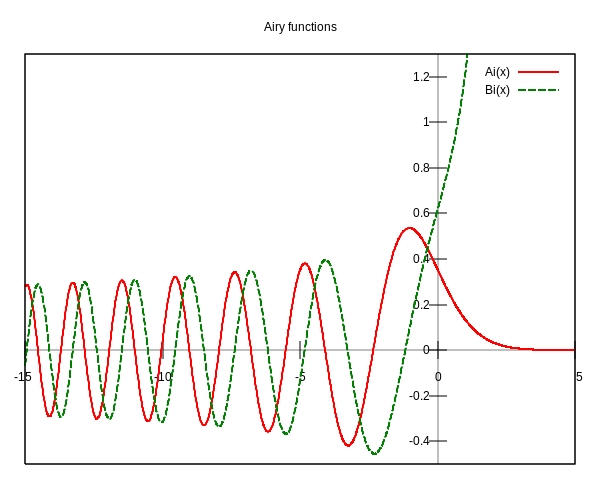
\includegraphics[scale=0.6]{Pictures/Airy_plot.svg.png} 
\end{center}
\caption{Graphique des deux solutions linéairement indépendantes de l'équation d'Airy, notées $Ai(x)$ et $Bi(x)$.
}
\label{fig:Airy}
\end{figure}

Soit un particule de masse $m$ soumis à la pesanteur, et limité à la région des $z$ positifs. 
Le potentiel que voit la particule est donc
\begin{eqnarray}
V(z)&=& mgz \quad z>0 \nonumber\\
&=& +\infty \quad z\leq 0 \ .
\end{eqnarray}

La trajectoire classique de cette particule est  une série de chutes libres, séparées par des rebonds lorsque la particule atteint $z=0$ lorsque sa vitesse change de signe).

Classiquement l'énergie minimale de cette particule est $E=0$, correspondant à la particule au repos en $z=0$.

Nous désirons étudier les états stationnaires de ce système $\psi(z)$, solutions de l'équation de Schrödinger
\begin{equation}
\left( -\frac{\hbar^2}{2m}\partial_z^2 + V(z) \right) \psi (z)= E \psi (z)\ .
\label{Eq:Schg}
\end{equation}
et en particulier déterminer l'énergie de l'état fondamental.

\begin{enumerate}

\item
Utilisez le principe d'incertitude pour estimer la hauteur moyenne $\langle z  \rangle$ à laquelle se trouve la particule, et son énergie, lorsqu'elle est dans l'état d'énergie minimum, en fonction de $m$, $g$, $\hbar$. Donner les valeurs de cette hauteur moyenne et de cette énergie dans le cas d'un électron dans le champ de pesanteur terrestre.

\item
Quelle sont les conditions que doit satisfaire $\psi(z)$ en $z=0$ et pour $z\to +\infty$ pour être un état propre de l'Hamiltonien?

\item
Faites un changement de variables 
\begin{equation}
z \to x = \alpha (z-z_0)
\end{equation}
pour ramener l'équation Eq. (\ref{Eq:Schg}) à la forme
\begin{equation}
\partial_{x}^2  \psi (x) - x \psi (x)= 0 .
\label{Eq:SchgB}
\end{equation}

\item 
Quelles sont les conditions que doit obéir $\psi(x) $ pour être un état propre de l'Hamiltonien?

\item
L'équation  Eq. (\ref{Eq:SchgB}) est connue sous le nom d'équation d'Airy. Les deux solutions linéairement indépendantes de l'équation d'Airy sont notées $Ai(x)$ et $Bi(x)$. Leur graphique est donné dans la figure. 

Pour $x$ grand positifs, ces fonctions se comportent comme 
\begin{eqnarray}
Ai(x)  &\simeq& a e^{- \frac{2}{3} x^{3/2}} \quad \text{lorsque } x\gg 0 \quad \text{(décroit exponentiellement)}\\
Bi(x)  &\simeq&  b e^{+ \frac{2}{3} x^{3/2}} \quad \text{lorsque } x\gg 0 \quad \text{(croit exponentiellement)}
\end{eqnarray}
avec $a$ et $b$ des constantes.

Ces deux fonctions oscillent pour $x$ négatifs. Les premiers zéros de $Ai(x)$ sont approximativement $-2.33811$, $-4.08795$, $-5.52056$.
Les premiers zéros de  $Bi(x)$  sont approximativement $-1.17371$,  $ -3.27109$, $-4.83074$.

Utilisez ces résultats pour donner l'énergie $E_0$ de l'état fondamental de $H$ et l'énergie $E_1$ du premier état excité, en fonction de $m$, $g$, $\hbar$.
Comparez avec votre estimation obtenue au point 1.

\end{enumerate}